\section{Multi-wavelength OWC system}
\label{sec:wdmSystem}
\graphicspath{{_System/figures_wdm/}}

Most VLC systems constructed to date focus on using a broad visible band generated by phosphor-converted LEDs, or by filtering to isolate the blue component from these sources. Multi-wavelength systems\footnote{This work is published in peer--reviewed IEEE conference proceeding \cite{but14c}.} consider additional wavelength bands that are combined to produce the desired lighting output along with OWC. Color combining, or mixing, realizes desired color temperature and intensity and represents a form of  wavelength-division multiplexing. This section investigates the relationships between the colors comprising the lighting source for a range of lighting states, the spectral separation of communication channels, the relative intensities required to realize lighting states, how modulation can be most effectively mapped to the available color channels, and the design of an optical filtering approach to maximize SNR while minimizing crosstalk at the receiver. Simulation results based on a three colored VLC system are discussed using O-OFDM for each color. It is shown that the system is the most power efficient at 6250 K correlated color temperature, with transmitter spectral spread of 5 nm and filter transmittance width of 40 nm.

\subsection{WDM system outline}
\label{subsec:wdmSystemWdm}

Different colors including shades of white for illumination on the black body radiation curve can be produced by mixing different amounts of narrow-band SPDs emitted by different sources. The ability to combine multiple narrow-band sources to generate white light also provides the benefit of being able to transmit concurrent information streams over different color groups; thus enabling WDM. As discussed before, the MIMO OWC system can be represented by the model in Eq. \eqref{eqWDMModel}
\begin{equation}
	\vm{Y} = \vm{H}\vm{X} + \vm{W}
	\label{eqWDMModel}
\end{equation}
$\vm{X}$ is a vector containing radiant fluxes emitted by $N_{\text{tx}}$ transmitting elements over different colors. $\vm{H}$ is $N_{\text{rx}}\times N_{\text{tx}}$ dimensional channel matrix where each element $h_{ij}$ represents channel gain from transmitter $j$ to receiver $i$. \vm{W} is the $N_{\text{rx}}$ dimensional AWGN vector. \vm{Y} is the vector of $N_{\text{rx}}$ received electrical signals.

Lasers and LEDs produce a much smaller SPD spread as compared to incandescent and fluorescent sources and are thus preferable for WDM. LED emission can be modeled with a Gaussian distribution as in Eq. \eqref{eqSPDGaussian} while laser emission can be modeled with a Lorentzian distribution as in Eq. \eqref{eqSPDLorentzian}. Equations in \eqref{eqSPD} model emission spectra for the $j^{th}$ transmitting element.
\begin{subequations}
\begin{align}
S_j(\lambda) &= \frac{1}{\sqrt{2\pi\sigma_j^2}}exp\left[-\frac{(\lambda-\lambda_j)^2}{2\sigma_j^2}\right]\label{eqSPDGaussian}\\
S_j(\lambda) &= \frac{1}{\pi}\frac{0.5\Gamma_j}{(\lambda-\lambda_j)^2 + (0.5\Gamma_j)^2}\label{eqSPDLorentzian}
\end{align}
\label{eqSPD}
\end{subequations}
where $\lambda_j$ is the dominant wavelength of emission, $\sigma_j$ is the measure of spread (deviation) from the dominant wavelength for the Gaussian model, and $\Gamma_j$ is the full width at half maximum (FWHM) from the dominant wavelength for the Lorentzian model. At small SPD spread, most of the optical power is emitted at the dominant wavelength. At larger SPD spread the optical power is distributed across a larger wavelength range and starts overlapping across different transmitting elements, thus causing interference. White light with SPD $W(\lambda)$ can be generated by combining emissions from different transmitting elements. The chromaticity coordinates for $W(\lambda)$ can be then be computed by using Eqs. \eqref{eqTXYZ}--\eqref{eqWXY} as described in section \ref{sec:cskNonlinear}.

Illumination color to rendered by luminaires is specified by correlated color temperature (CCT) in Kelvin units. To understand CCT, consider spectral radiance of a black body heated to temperature $T$ Kelvin as stated by Planck's law and given by
\begin{equation}
\label{eqPlanck}
	 S(\lambda) = \frac{2hc^2}{\lambda^5\left[\text{exp}\left(\frac{hc}{\lambda kT}\right)-1\right]}
\end{equation}
where $h$ is the Planck's constant, $c$ is speed of light, and $k$ is Boltzmann's constant. Replacing $W(\lambda)=S(\lambda)$ in Eqs. \eqref{eqTXYZ}-- \eqref{eqWXY} chromaticity coordinates $[x,y]$ associated with a black body heated to temperature $T$ can be computed. In this context $T$ is known as the CCT for color represented by $[x,y]$. Recall that two different SPDs can generate the same chromaticity coordinates due to the principle of metamerism. A luminaire specified to render a CCT value will generate an SPD that is metamerically equivalent to the SPD emitted by a black body heated to specified CCT.

Traditionally luminaires have been specified to generate a certain CCT with colors at lower temperature appearing (ironically) warmer than those at higher temperatures. It is practical to generate colors off the black body radiation curve using different colored sources. This analysis considers only the colors generated on the black body radiation curve. As the CCT changes from a lower value to a higher value, the optical power available to transmit information on any color channel varies thus affecting the overall communication performance.

Optical filters can be manufactured to permit narrow-bandpass filtering using plasmonics \cite{xu10a,yok12a}. Broad-bandpass optical filters that make use of interference are widely available. The transmittance of these filters can be modeled as Lorentzian functions of wavelength. The choice of the filter FWHM is a tradeoff to collect the maximum signal while rejecting interference and background illumination.

Responsivity of the receiving elements also affects the aggregate system performance. It depends on the quantum efficiency of the material of sensor. Reference \cite{gha12a} computes responsivity as
\begin{equation}
\label{eqResponsivity}
	 R(\lambda) = \frac{\xi\lambda}{1240}
\end{equation}
where $\xi$ is the quantum efficiency of the material, and $\lambda$ is wavelength of interest. For equal signal radiant flux, signals that span wavelength ranges with lower responsivity will perform poorly as compared to the rest. 

Optical spectrum outside the visible range like infrared (IR) and ultraviolet (UV) spectrum can also be utilized for WDM. IR and UV do not generate chromatic response on human eye and thus do not contribute to visible illumination. Thus, as long as their emissions satisfy eye and skin safety regulations, using this additional optical spectrum can only boost the channel capacity.

%%%%%%%%%%%%%%%%%%%%%%%%%% SIMULATION %%%%%%%%%%%%%%%%%%%%%%%%%%
\subsection{WDM system performance}
\label{subsec:wdmSystemAnalysis}
This subsection studies how the choice of design parameters like illumination CCT, transmitter SPD, and filter FWHM affect the performance of a multi-wavelength VLC system. Three transmitting elements with Gaussian emission spectrum at dominant wavelengths of red (627 nm), green (530 nm) and blue (470 nm) are selected. Using these transmitting elements, CCT range of [2500 7000] K is sought. SPD spread within [5 50] nm is considered. \figurename{ \ref{fig:LEDSPD}} illustrates normalized SPDs needed to achieve the range of CCTs for transmitting elements with 5 nm spread.

\begin{figure}[!t]
	\centering
		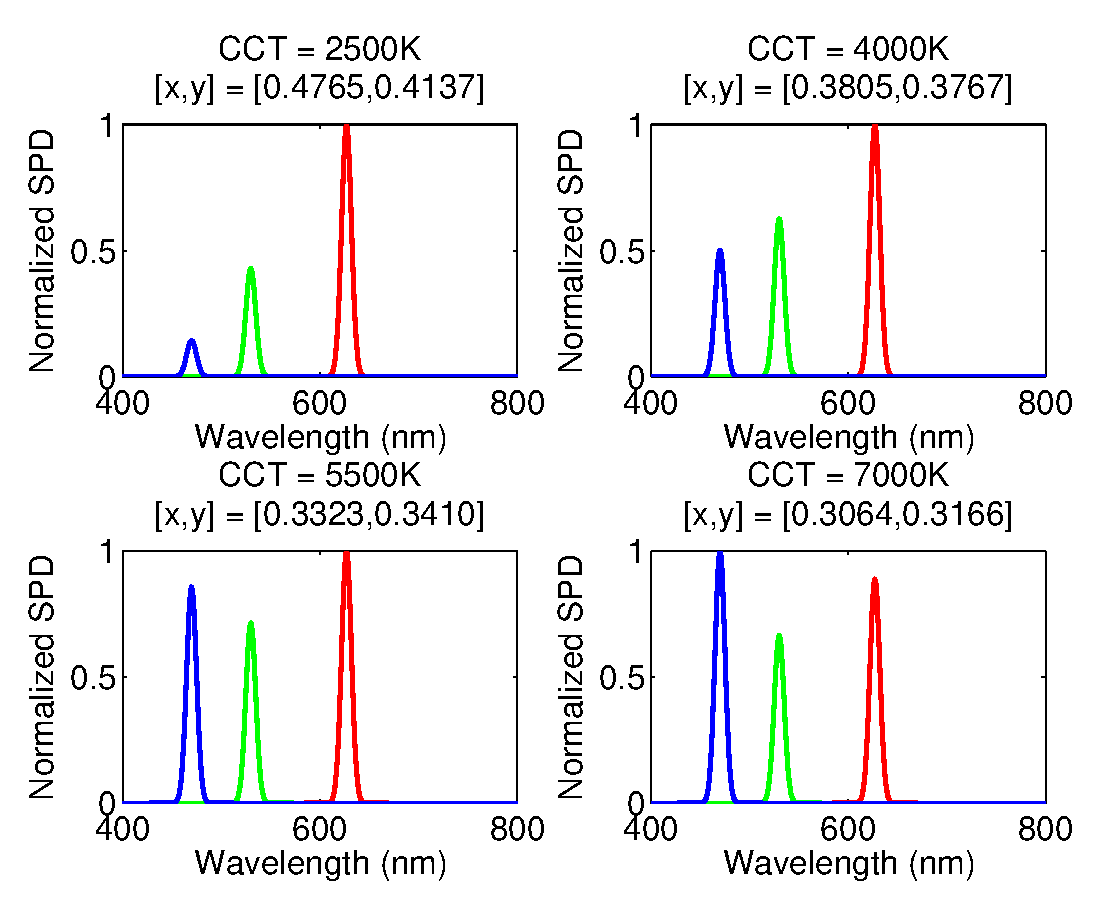
\includegraphics[trim={0.05in 0.05in 0.05in 0.0in}, clip=true, width=4.5in]{LEDSPD.eps}
	\caption{Transmitting element normalized spectral power distribution}
	\label{fig:LEDSPD}
\end{figure}

Unique $t_{\text{R}}:t_{\text{G}}:t_{\text{B}}$ ratios are generated after varying the tristimulus values in the range [0 1] in 0.1 unit steps. Chromaticity coordinates for resulting SPDs are calculated. An initial characterization step generates a pre--populated table consisting of the tristimulus values and corresponding chromaticity coordinates. Chromaticity coordinates for each CCT are also pre--computed. From the pre--computed table, the tristimulus values that achieve the closest chromaticity are selected. The SPD is then scaled to achieve target illumination (400 lx) at the receiver that is located at a distance of 2 m from the transmitter. The surface normals of the transmitter and receiver are assumed to be parallel.

Optical filter's passband can be designed to center on the transmitting elements' dominant wavelengths. Optical filters for the simulation are modeled to have Lorentzian transmittance with ideal value $1$ at the dominant red, green and blue wavelengths mentioned above. Filter transmittance as a function of wavelength is illustrated in \figurename{ \ref{fig:FiltTr}}. Filter FWHM considered for the analysis lie in [1 250] nm range.

\begin{figure}[!t]
	\centering
		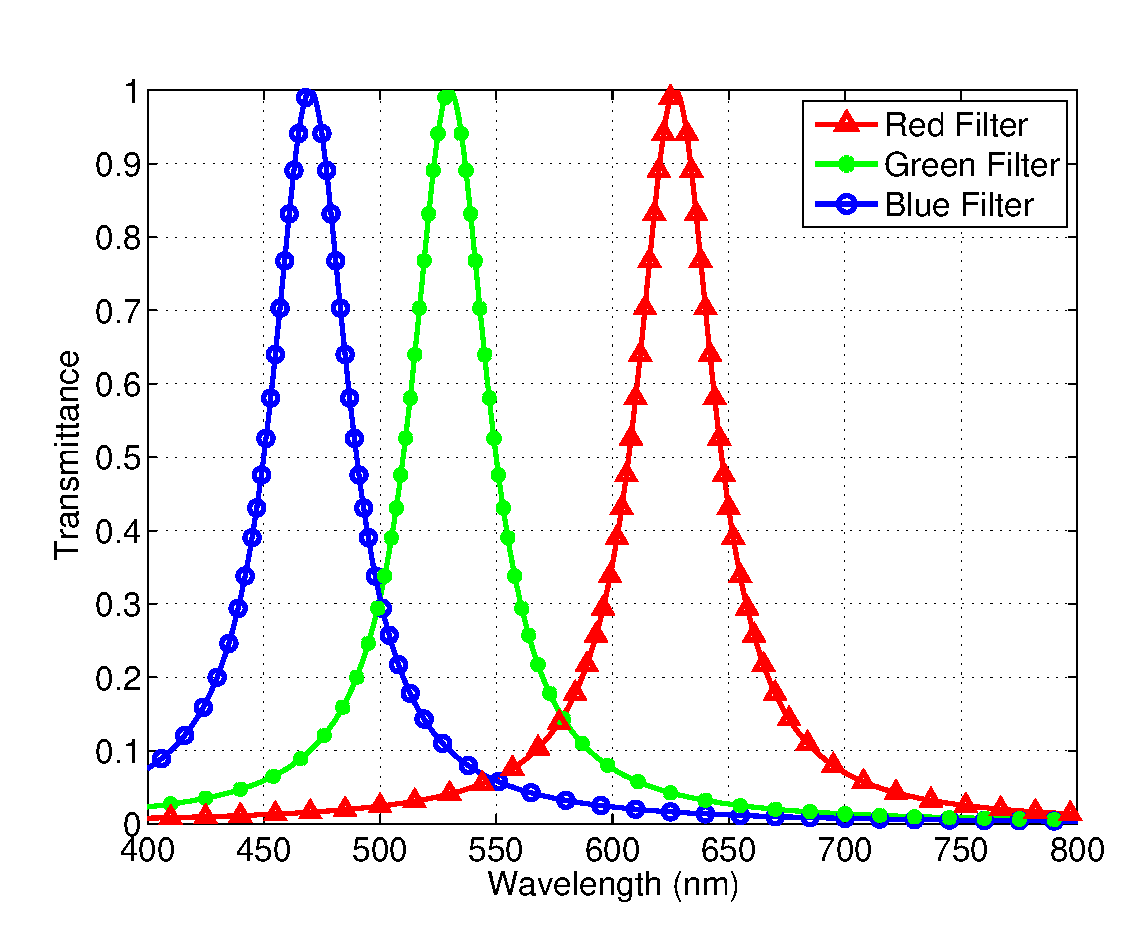
\includegraphics[trim={0.15in 0.05in 0.05in 0.35in}, clip=true, width=4.5in]{FiltTr.eps}
	\caption{Filter transmittance for FWHM = 40 nm}
	\label{fig:FiltTr}
\end{figure}

% online source \cite{qeff}
The receiver sensor is assumed to be made of silicon. The assumed quantum efficiencies and responsivity of the sensor taken from online source is illustrated in \figurename{ \ref{fig:RecvResp}}. The responsivity near the blue wavelength is about 0.29 A.W$^{-1}$ and increases steadily to about 0.46 A.W$^{-1}$ near the red before rapidly reducing as the energy of the incident photon approaches the bandgap energy of silicon.

To analyze the system performance with reasonable number of iterations, transmitting and receiving elements are restricted to the same deviations about their respective means. A random bit stream is then generated. Bits for each link are then communicated using asymmetrically clipped offset and DC-biased optical orthogonal frequency division multiplexing (ACO-OFDM and DCO-OFDM). Details on these optical OFDM techniques can be found in references \cite{car96a,arm06a}. For this simulation, ACO-OFDM and DCO-OFDM are implemented with 64 sub-carriers and 64-QAM and 8-QAM modulation, respectively. This ensures that both schemes achieve similar bits/symbol with ACO-OFDM achieving 96 bits/symbol and DCO-OFDM achieving 93 bits/symbol. The DC level on each link is set to ensure the desired CCT is achieved at the 400 lx illumination level. This generates the transmit vector $\vm{X}$. 

\begin{figure}[!t]
	\centering
		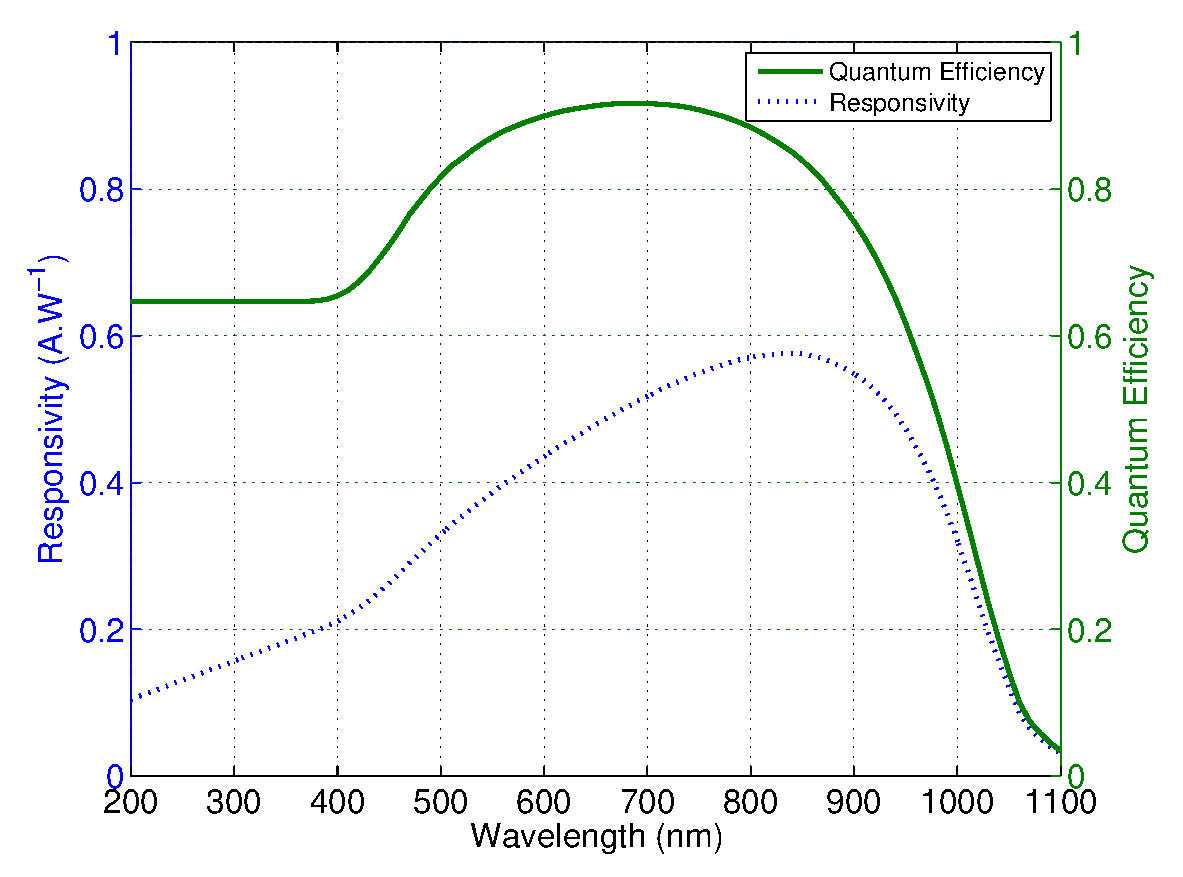
\includegraphics[trim={0.15in 0.05in 0.05in 0.0in}, clip=true, width=4.5in]{RecvResp.eps}
	\caption{Receiver quantum efficiency and responsivity}
	\label{fig:RecvResp}
\end{figure}

Having established $N_{\text{tx}} = 3$ transmitting and $N_{\text{rx}} = 3$ receiving elements, the $3\times 3$ channel matrix $\vm{H}$ can be computed. AWGN vector $\vm{W}$ is generated and is then added to the transmitted vector. With the knowledge of the transmitted signal power and by varying the receiver noise, simulations over a range of $\text{SNR}^{\text{tx}}_{\text{avg}}$ as defined in Eq. \eqref{eqOSMSNRTX} are carried out. Vector \vm{Y} then collects the received signal and the added noise and interference. The least squares estimate of the transmitted signal vector is computed as
\begin{equation}
	\label{eqXhat}
	\hat{\vm{X}} = (\vm{H}^{*}\vm{H})^{-1}\vm{H}^{*}\vm{Y}
\end{equation}

An estimate of the transmitted optical OFDM frame for each color is obtained by aggregating least squares estimates of the received signal vectors. Further signal processing on each optical OFDM frame gets an estimate of the transmitted QAM symbol. Decoding the QAM symbols provides an estimate of the transmitted bits. BER is then calculated by comparing the transmit and estimated bit--streams.


%\begin{figure*}[!t]
%\centerline{\subfloat[Most power efficient operation point]{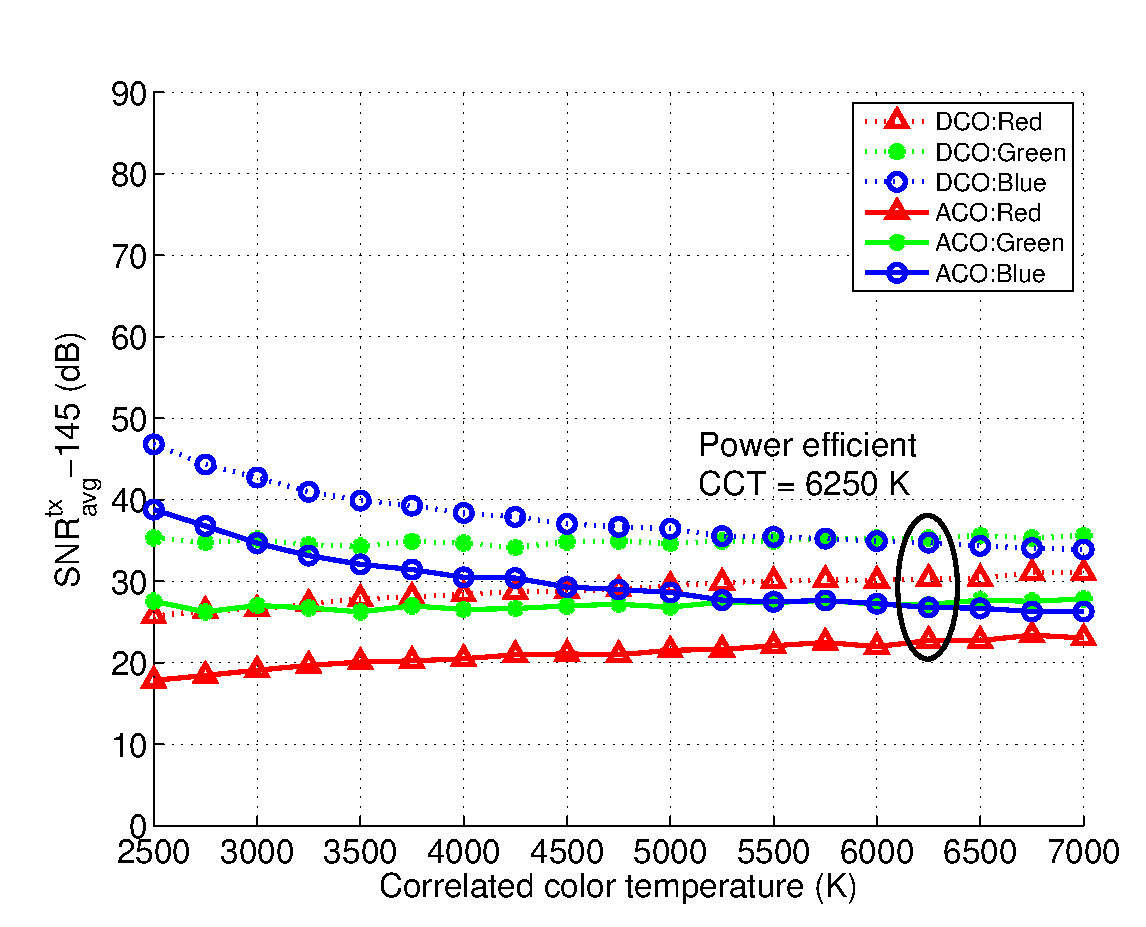
\includegraphics[trim={0.15in 0.05in 0.05in 0.35in}, clip=true, width=2.9in]{SNRvsCCT.eps} \label{subfig:SNRvsCCThigh}}
%\hfill
%\subfloat[High inter-channel interference]{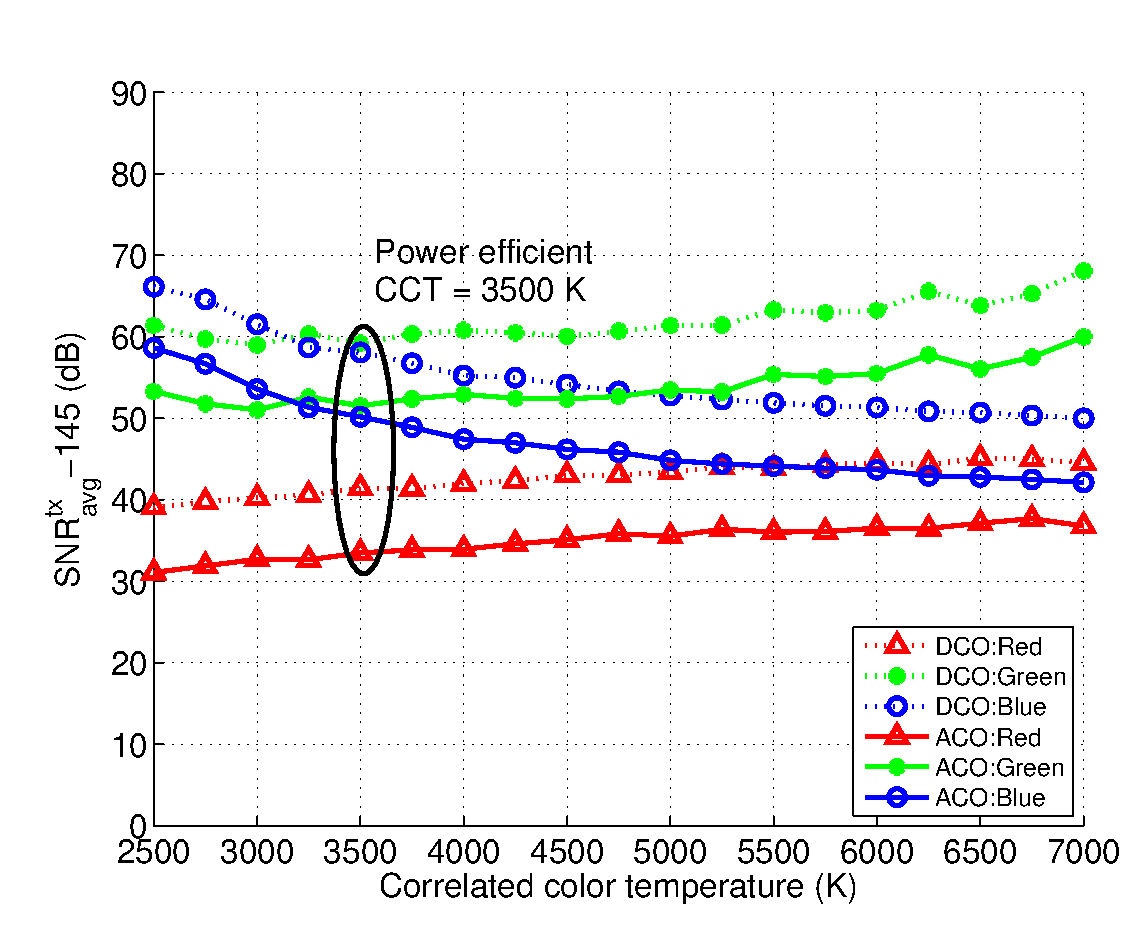
\includegraphics[trim={0.15in 0.05in 0.05in 0.35in}, clip=true, width=2.9in]{SNRvsCCT2.eps} \label{subfig:SNRvsCCTlow}}}
%\caption{$\text{SNR}^{\text{tx}}_{\text{avg}}$ vs correlated color temperature to achieve BER $\leq 10^{-3}$ \newline(a) Transmitter: $\sigma_r = \sigma_g = \sigma_b = 5$ nm; Filter: $\Gamma_r = \Gamma_g = \Gamma_b = 40$ nm (b) Transmitter: $\sigma_r = \sigma_g = \sigma_b = 50$ nm; Filter: $\Gamma_r = \Gamma_g = \Gamma_b = 250$ nm}
%\label{fig:SNRvsCCT}
%\end{figure*}
%\global\let\figone\relax


%%%%%%%%%%%%%%%%%%%%%%%%%%%% RESULTS %%%%%%%%%%%%%%%%%%%%%%%%%%%
%\subsection{Results and Discussion}
%\label{subsec:wdmSystemResults}
\afterpage{
\begin{figure}[!t]
	\centering
		\begin{subfigure}{\textwidth}
		\centering
			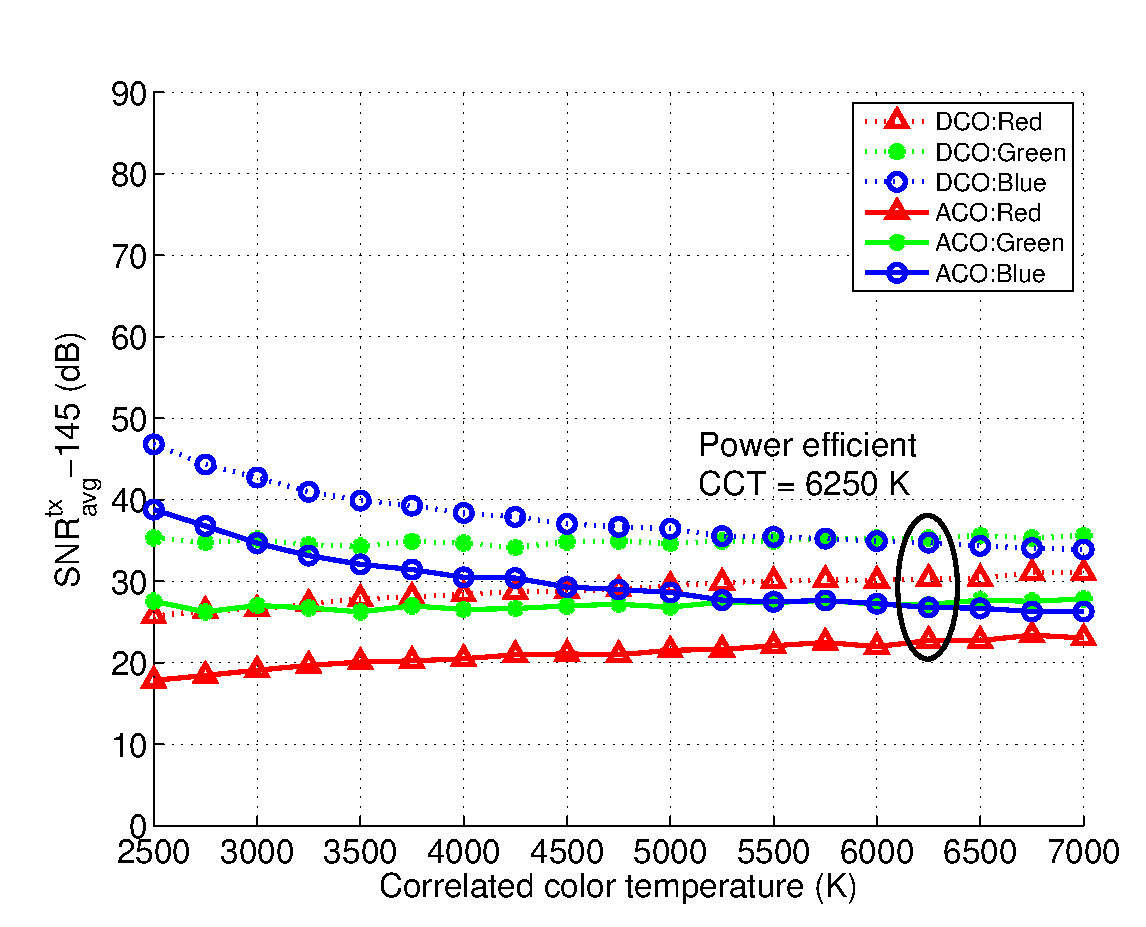
\includegraphics[trim={0.15in 0.05in 0.05in 0.35in}, clip=true, width=0.7\textwidth]{SNRvsCCT.eps}
			\caption{Most power efficient operation point}
			\label{subfig:SNRvsCCThigh}
		\end{subfigure}
		%\hfill
		\begin{subfigure}{\textwidth}
		\centering
			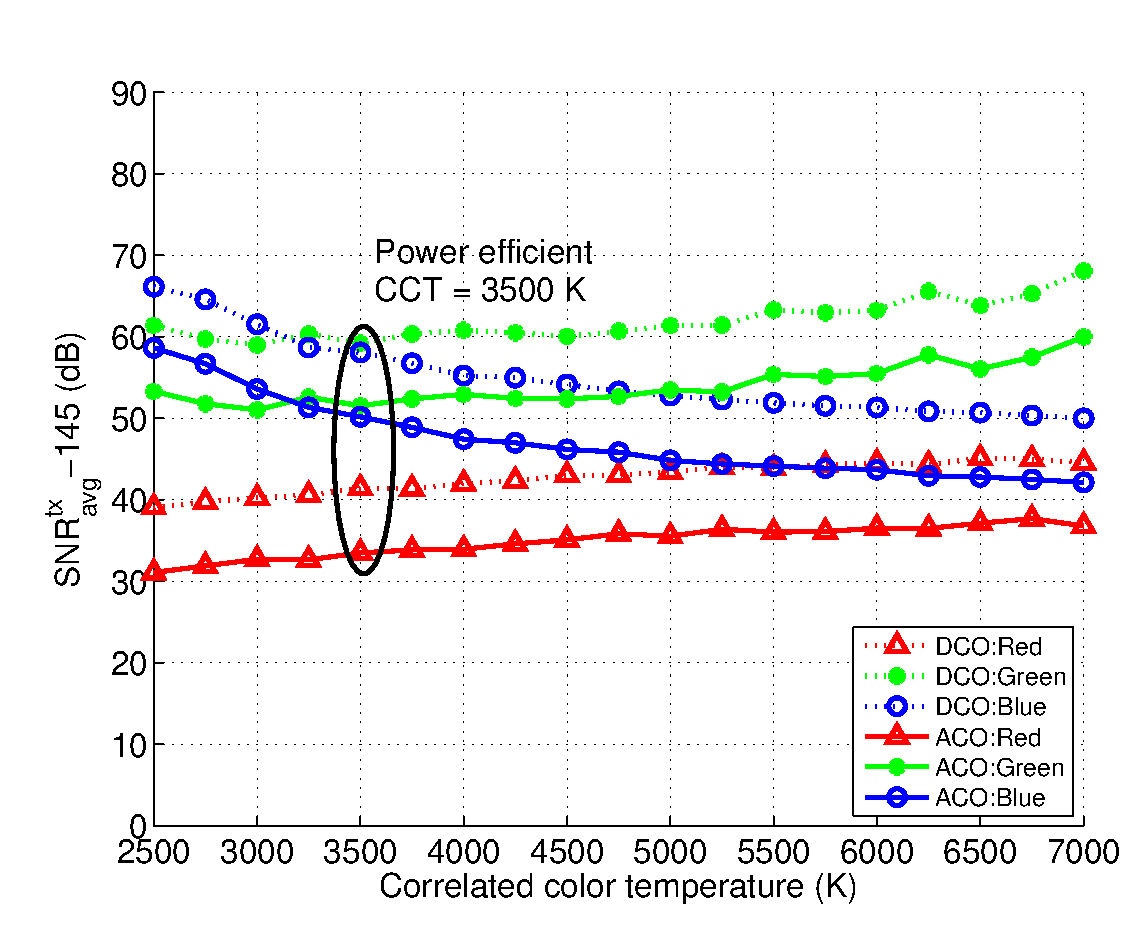
\includegraphics[trim={0.15in 0.05in 0.05in 0.35in}, clip=true, width=0.7\textwidth]{SNRvsCCT2.eps}
			\caption{High inter-channel interference}
			\label{subfig:SNRvsCCTlow}
		\end{subfigure}
	\caption[SNR vs CCT for multi--color system]{$\text{SNR}^{\text{tx}}_{\text{avg}}$ vs correlated color temperature to achieve BER $\leq 10^{-3}$ \newline(a) Transmitter: $\sigma_r = \sigma_g = \sigma_b = 5$ nm; Filter: $\Gamma_r = \Gamma_g = \Gamma_b = 40$ nm (b) Transmitter: $\sigma_r = \sigma_g = \sigma_b = 50$ nm; Filter: $\Gamma_r = \Gamma_g = \Gamma_b = 250$ nm}
\label{fig:SNRvsCCT}
\end{figure}
}
For each unique configuration yielded by varying the parameters, BER versus $\text{SNR}^{\text{tx}}_{\text{avg}}$ is empirically determined using monte-carlo simulations. Based on the simulation setup, the path-loss from the transmitting elements to the receiving elements is about 145 dB. To plot the change in system performance when each parameter is varied, the minimum $\text{SNR}^{\text{tx}}_{\text{avg}}$ needed to achieve target BER $\leq 10^{-3}$ is selected. Since ACO-OFDM is more power efficient compared to DCO-OFDM, for all the cases discussed below, ACO-OFDM needs lower transmit signal power to achieve the target BER as compared to DCO-OFDM.

The change in performance of the red, green and blue links as the CCT is varied from 2500 K to 7000 K is shown in \figurename{ \ref{fig:SNRvsCCT}}. At 2500 K, the SPD has a greater contribution from red, then green and then blue. Thus the red link achieves target BER at lower transmitted signal power. As the CCT increases, relative signal power from the red link decreases, that of the green remains similar, and that of the blue increases. Thus, with increase in CCT, the amount of aggregate transmit flux needed to achieve target BER from the red link starts increasing, that of the green remains relatively unchanged, while that of the blue decreases. For the specified multi-wavelength system, CCT = 6250 K provides the most power efficient operating point as illustrated in \figurename{ \ref{subfig:SNRvsCCThigh}}. Increasing the transmitting elements' SPD or the filter FWHM introduces increasingly more ICI. This causes the most power efficient operating point to shift towards CCT = 3500 K but with greater power requirements as seen in \figurename{ \ref{subfig:SNRvsCCTlow}}.

\begin{figure}[!t]
	\centering
		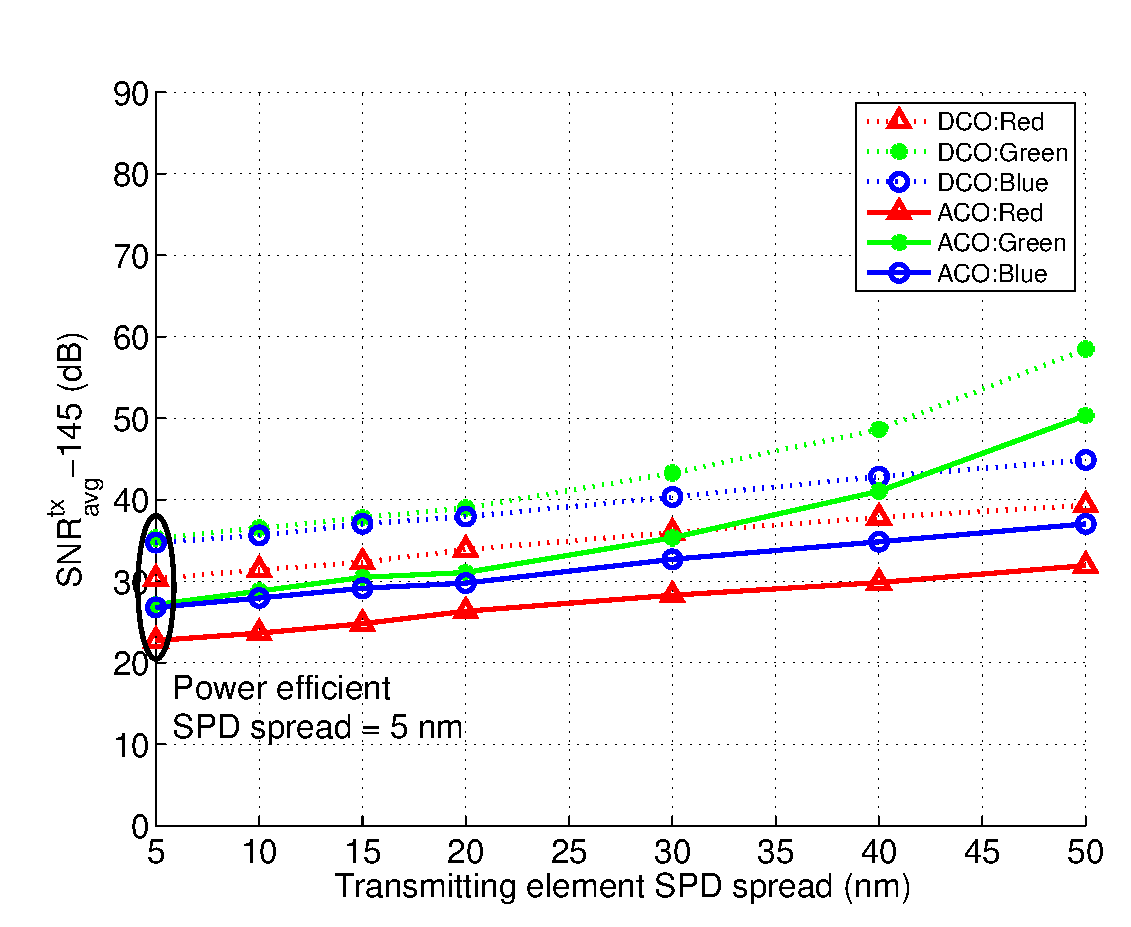
\includegraphics[trim={0.15in 0.05in 0.05in 0.35in}, clip=true, width=0.7\textwidth]{SNRvsLEDSD.eps}
	\caption[SNR vs transmitter SPD spread for multi--color system]{$\text{SNR}^{\text{tx}}_{\text{avg}}$ vs transmitting element SPD spread to achieve BER $\leq 10^{-3}$\newline Filter: $\Gamma_r = \Gamma_g = \Gamma_b = 40$ nm; CCT = 6250 K}
	\label{fig:SNRvsLEDSD}
\end{figure}

The change in performance of the red, green and blue links as the transmitting element SPD spread is varied from 5 nm to 50 nm is shown in \figurename{ \ref{fig:SNRvsLEDSD}}. As the SPD spread is increased, the performance of all three links degrade. This can be attributed to two factors. Initially, as the signal power is distributed across a larger wavelength range, with the filter transmittance function remaining the same, increasingly more signal gets rejected by the filter. Thus the receiver collects a smaller fraction of the signal power, degrading the performance. Secondly, as the individual SPDs spread enough, they start overlapping and causing ICI. The effect of ICI is more pronounced on the green link because it gets interference from both, red and blue. Thus transmitter consisting of transmitting elements with narrower emission spectra are more power efficient efficient than those with wider emission spectra. Experiments in reference \cite{neu11a} qualitatively measure color perception for illumination with narrow-band sources and find lasers could be used for general lighting. However, it is also commonly believed that sources with spiky emission spectra do not produce good quality of illumination because objects with reflectance spectra lying outside the spikes in the illumination spectra will be perceived to be poorly lit. The choice of the transmitting elements' SPD spread would be a tradeoff between the communication and illumination performance. For the specified multi-wavelength system, SPD spread = 5 nm provides the most power efficient operating point.

\begin{figure}[!t]
	\centering
		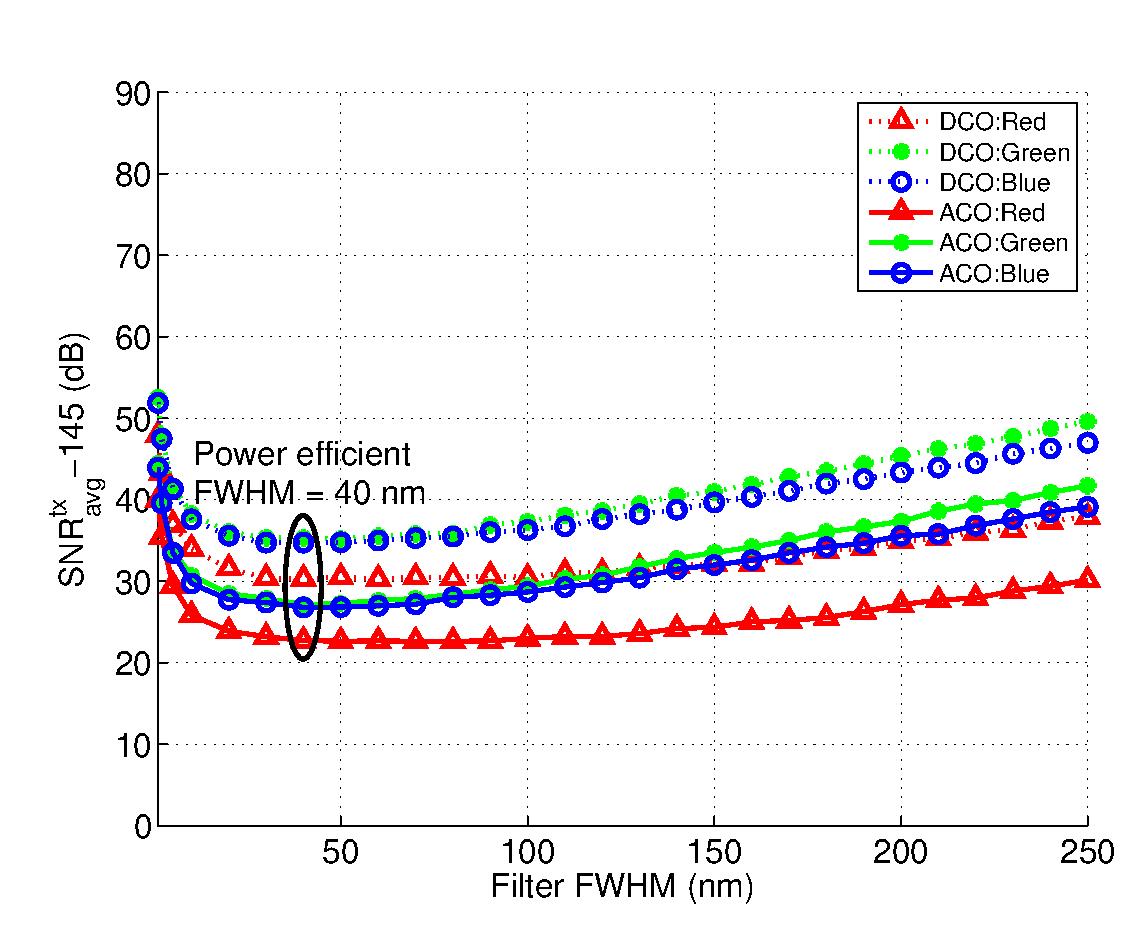
\includegraphics[trim={0.15in 0.05in 0.05in 0.35in}, clip=true, width=0.7\textwidth]{SNRvsFLTWID.eps}
	\caption[SNR vs filter FWHM for multi--color system]{$\text{SNR}^{\text{tx}}_{\text{avg}}$ vs filter FWHM to achieve BER $\leq 10^{-3}$\newline Transmitter: $\sigma_r = \sigma_g = \sigma_b = 5$ nm; CCT = 6250 K}
	\label{fig:SNRvsFLTWID}
\end{figure}

The change in performance of the red, green and blue links as the receiving element filter FWHM is varied from 1 nm to 250 nm is shown in \figurename{ \ref{fig:SNRvsFLTWID}}. As the filter FWHM increases, initially the system performance improves significantly. At these lower FWHM ranges, the filters transmit a smaller fraction of the signal to the sensors and thus performance is limited by the amount of signal power collected for each link. At higher FWHM ranges, along with additional signal, the filters permit increasingly more ambient light and interference from neighboring links, thus degrading the performance. For the specified multi-wavelength system, filter FWHM = 40 nm provides the most power efficient operating point.

In this section, design paradigm for a multi-wavelength VLC system in the context of variable illumination constraints is presented. VLC system performance is characterized for variations in illumination CCT, transmitter SPD spread, and the receiver filter transmittance FWHM. For the three colored system considered, the blue and the green links pose the performance bottlenecks because of the relatively lower contribution to the SPD and lower PD responsivity as compared to the red. As the ICI increases, the most power efficient CCT shifts towards lower temperatures. Transmitting elements with the smallest spectral spread provide the most power efficient operating point. The effect of increase in spectral spread is most pronounced in the green link because it suffers the most from interference from the blue and red links. Filters with narrow transmittance FWHM reject a lot of the signal power while filters with a broad transmittance FWHM accept a lot of interference. Both of these affect the power efficiency of the system. For the setup considered, the most power efficient operating point is for ACO-OFDM at CCT = 6250 K, transmitting element SPD spread = 5 nm, and filter FWHM = 40 nm.






